\chapter{container 라이브러리}

\section{솔루션 준비}

\subsection{프로젝트 생성}

gsp\_library C++ 콘솔 프로젝트를 만듭니다. 해당 폴더의 파일들을 적절하게 정리합니다. 

저는 gsp\_library 솔루션과 프로젝트를 만들었습니다. gsp\_library.cpp 파일의 
main을 doctest에서 제공하는 main의 내용으로 교체합니다. 

내용은 다음과 같습니다. 

\begin{lstlisting}[language=c++, caption={doctest main 내용}]
    #define DOCTEST_CONFIG_IMPLEMENT
    #include <doctest/doctest.h>
    
    int main(int argc, char** argv) 
    {
      doctest::Context context;
    
      // exclude test cases with "math" in their name
      context.addFilter("test-case-exclude", "*math*"); 

      // stop test execution after 5 failed assertions
      context.setOption("abort-after", 5);              

      // sort the test cases by their name
      context.setOption("order-by", "name");  
    
      context.applyCommandLine(argc, argv);
    
      // overrides
      // don't break in the debugger when assertions fail
      // context.setOption("no-breaks", true);             
    
      int res = context.run(); // run

      // important - query flags (and --exit) rely on the user doing this
      if (context.shouldExit()) 
        return res;          // propagate the result of the tests
    
      int client_stuff_return_code = 0;

      // the result from doctest is propagated here as well
      return res + client_stuff_return_code; 
    }
\end{lstlisting}

\subsection{추가 설정}

프로젝트 속성의 vcpkg 항목에 Use Vcpkg, Use Static Libraries가 모두 예(Yes)로 설정되었느지 
확인해야 합니다. 또 C++ \textrightarrow 코드 생성에 DLL이 아닌 멀티쓰레드로 설정되었는지 
디버그와 릴리스 구성 모두 확인합니다. 왜냐하면 정적 라이브러리로 vcpkg에 설치하기 
때문입니다. 

빌드하고 실행해서 정상으로 동작하는지 확인합니다. 

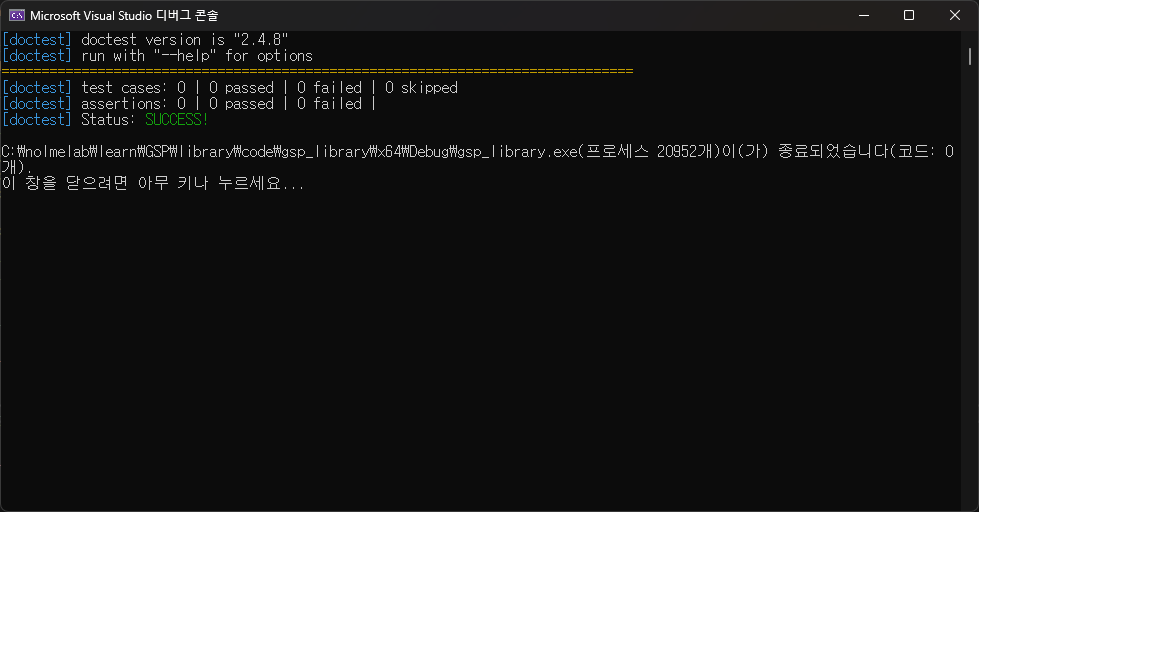
\includegraphics[scale=0.7]{build_execute}

\section{std::array}

고정길이 배열입니다. 템플릿으로 임의의 타잎의 오브젝트를 보관할 수 있습니다. 

\subsection{테스트 파일 만들기}

컨테이너들을 연습할 폴더 container를 만들고 폴더 안에 learn\_array.cpp 파일을 
추가하고 gsp\_library 프로젝트에 적절한 필터를 추가해서 넣습니다. 필터 명으로는 
폴더와 같은 container도 괜찮을 듯 합니다. 

\begin{lstlisting}[language=c++, caption={시작 골격}]
#include <doctest/doctest.h>

#include <array>

TEST_CASE("std::array")
{
  SUBCASE("basic interface")
  {

  }
}
\end{lstlisting}

\subsection{자료 읽기}

cppreference.com의 std::array 문서를 살펴봅니다. 

\begin{lstlisting}[language=c++, caption={타잎}]
  template<
    class T,
    std::size_t N
> struct array;
\end{lstlisting}

타잎 T와 크기 N을 받는 struct로 되어 있습니다. 

\begin{tcolorbox}
  std::array is a container that encapsulates fixed size arrays
\end{tcolorbox}

첫 문장이고 가장 중요한 내용입니다. 

그 이후에 이어지는 내용은 대체로 언어의 세밀한 정의와 관련된 부분이 나옵니다. 
처음 볼 때는 읽지 않아도 괜찮습니다. 




\subsection{코드 읽기}


